\documentclass[11pt]{article}
\usepackage{acl2014}
\usepackage{times}
\usepackage{url}
\usepackage{latexsym}
\usepackage{comment}
\usepackage{amsmath,amsthm,amssymb}
\usepackage{graphicx}
\usepackage{multirow}
\usepackage{color}

\DeclareMathOperator*{\argmin}{arg\,min}
\DeclareMathOperator*{\argmax}{arg\,max}

\newcommand{\mfar}[1]{\textcolor{blue}{\bf\small [#1 --MFAR]}}

\title{Improving Vector Space Word Representations\\
Using Prior Semantic Beliefs}


\begin{document}
\maketitle
\begin{abstract}
  Recent advances in vector space word representation learning has
  only exploited evidence from co-occurrence statistics in
  monolingual and multilingual text corpora. All such techniques are 
  consequentially unaware of the
  potentially crucial information present in handcrafted and automatically
  produced lexical ontologies that is not clearly evident from text. In this 
  paper, we propose a novel approach that combines distributional 
  information with additional knowledge from structured ontologies to 
  yield better quality semantic word representations
  than in isolation. We perform belief propagation on a graph constructed
  using available lexical ontologies to enforce connected words to
  have similar representations and show that our technique is applicable to
  different word vectors models across different languages and gives improvement
  in performance on a variety of evaluation tasks.
\end{abstract}

\section{Introduction}

The distributional hypothesis of \newcite{firth1957} \emph{``you shall know a word by the
company it keeps''} has led to a large interest in deriving various semantic representations
of words in terms of their frequent contextual patterns. One such representations is the vector
space model of word meaning representation that encodes a word in a vector of real numbers.
These word vectors can in turn be used for identifying semantically close word 
pairs~\cite{Turney:2006:SSR:1174520.1174523,Agirre:2009:SSR:1620754.1620758} or as features
in downstream applications like named entity recognition~\cite{turian:2010}.

%Data-driven learning of vector-space word embeddings that capture lexico-semantic 
%properties is a technique of central importance in natural language processing. 
It is possible to construct high-quality semantic vectors using cooccurrence 
statistics from a large corpus of text 
\cite{deerwester-90}, or using internal representations from neural 
network models of word sequences~\cite{Collobert:2008:UAN:1390156.1390177} to 
arrive at vector representations that capture co-occurence tendencies and meanings.
Variants of not only using co-occurrence statistics from monolingual corpora but looking
at alignments of words across languages~\cite{zou-EtAl:2013:EMNLP,hermann2014multilingual,faruqui-dyer:2014:EACL2014}
have been shown to perform better than their monolingual counterparts. Another variant of
constructing the word vectors considers the co-occurrence of words as determined by their
dependency syntax~\cite{Pado:2007:DCS:1268656.1268658}. 

In a similar spirit, we propose that
word vector representations can be further improved by looking at the neighboring words
in a lexical ontology. Lexical ontologies like the WordNet~\cite{miller:1995}, 
FrameNet~\cite{Baker:1998:BFP:980845.980860} or the Paraphrase 
database~\cite{ganitkevitch2013ppdb} contain words that are connected to other words in 
the same language through specific relations. These relations in turn determine the semantic
association between the words. This is an obvious source of information that has not been
exploited in creating word vectors so far. 

We present a graph-based learning framework which
uses the lexical ontologies to create a word graph (\S\ref{sec:graph}) where semantically associated words
are connected to each other. We then perform belief propagation on the graph which enforces
similar words to have similar word vector representations. Our method of incorporating prior
semantic beliefs can be used both while training (\S\ref{sec:improve-tr}) the word vectors or as a 
post-processing step (\S\ref{sec:post-proc}). 
We show that our method works well with
different types of word vector models (\S\ref{sec:vectors}) and gives substantial improvements on a 
variety of vector evaluations tasks (\S\ref{sec:eval}) while using different kinds of lexical ontologies (\S\ref{sec:onto}) across different languages (\S\ref{sec:multilingual}).

\section{Graph Encoding of Prior Beliefs}
\label{sec:graph}

\begin{figure*}[tb]
  \centering
  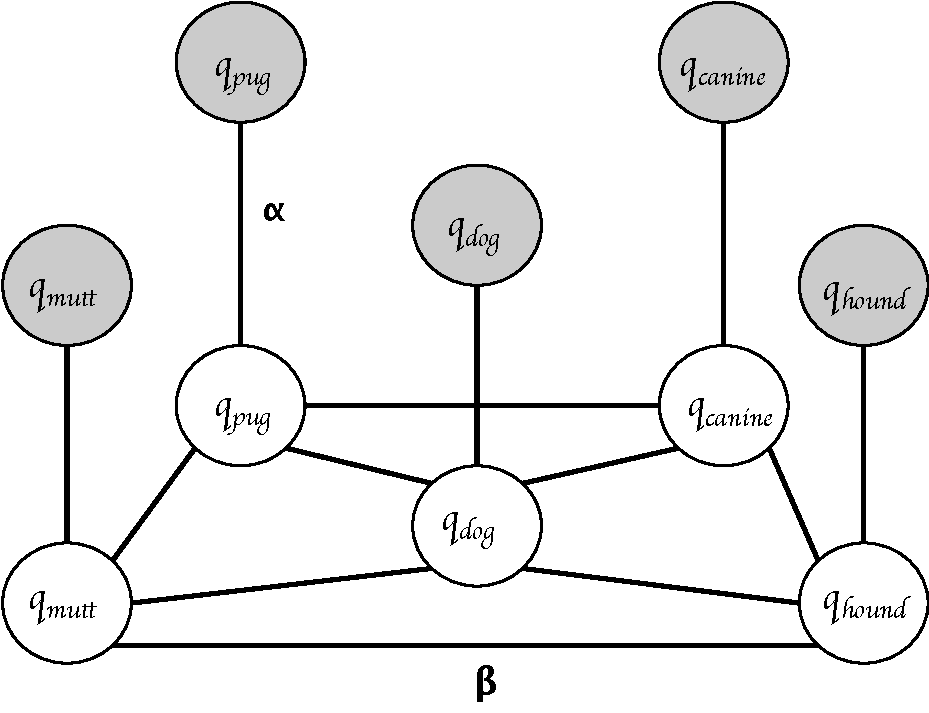
\includegraphics[width=\columnwidth]{diagram.pdf}
  \caption{Word graph with edges between related words showing the observed and the inferred word vector representations.}
  \label{fig:word-graph}
\end{figure*}

Let $W = \{w_1,...,w_n\}$ be the set of word types and $\Omega$ be an ontology that encodes a set of semantic relations between words in $W$. 
Specifically, we define $\Omega = (V_\Omega,E_\Omega)$ to be an undirected graph with vertices $V_\Omega = \{v_i | \  \forall \  w_i \in W\}$ and 
edges $E_\Omega = \{e_{ij}\}$ for every pair of words $(w_i,w_j)$ that are semantically linked according to some relation.
%For now we consider all the word types to be unambiguous in meaning, although later we will see how 
%our model also lets us derive word embeddings for different senses of 
%word types. 
Since majority of the existing word representation models ignore word-senses,
we consider $\forall i, w_i$ to be unambiguous word-types.

Then, given a set of vectors $\hat{Q} = \{\hat{q}_i | \  \forall \  w_i \in W\}$ that have been learned from any of the currently available
methods to obtain word vector representations, our objective is to learn a set of vectors $Q = \{q_i | \  \forall \  w_i \in W\}$ that are 
consistent with both $\hat{Q}$ and $\Omega$ by a notion of distance metric between vectors. Figure~\ref{fig:word-graph} shows a small word graph with such edge 
connections. The layer containing vectors $Q$ and vectors $\hat{Q}$ can be seen as the unobserved and observed layers in a Markov Random Field 
\cite{kindermann80mrf}. We initialize the vectors in $Q$ to be equal to the vectors in $\hat{Q}$.
and then perform inference to obtain the unobserved (and improved) word representations $\hat{Q}$.

We define the distances between any two nodes as the euclidean distance
\footnote{Using cosine similarity as distance yields the same update equation for vectors of unit length}
 between them, thus forcing 
similar nodes to have similar vector representations. Since, we want the inferred word vector to be
associated both with its observed value $\hat{q}_i$ and its neighbors 
$q_j, \forall ij \in E_{\Omega}$, the clique potential becomes:
\begin{equation}
  \label{equ:eucl}
  \displaystyle C(Q) = \sum_{i=1}^n \left[ \alpha \lVert q_i - \hat{q_i} \rVert^2 + \sum_{ij \in E_{\Omega}} \beta_{ij} \lVert q_i - q_j \rVert^2 \right]
\end{equation}
where, $\beta_{ij}$ is the weight of the edges connecting $i,j$ and $\alpha$ is a hyper-parameter to control the degree of deviation of the word 
vector from its observed value. Equation~\ref{equ:eucl} is a convex optimization problem and a close formed solution does exist but practically is intractable to compute. Thus, we take the gradient of equation~\ref{equ:eucl} with respect to the parameters to be optimized, namely: $\forall i, q_i$ and equate it to zero get the following update for $q_i$:
\begin{equation}
  \label{equ:update-vector}
q_i = \frac{\sum_{j, ij \in E} \beta_{ij} q_j + \alpha \hat{q_i}}{\sum_{j, ij \in E} \beta_{ij} + \alpha}
\end{equation}
We run this procedure for $10$ iterations to achieve convergence.

\section{Word Vector Representations}
\label{sec:vectors}

We show that our method to improve word vectors can be used both as a 
post-processing step or during training.
For the post-processing step, we take word vectors available from four different 
models and enrich them using
equation~\ref{equ:update-vector}. To show that our model can also be used 
while training the word vectors, we train the log-bilinear word embeddings model (\S\ref{sec:lbl}).

\subsection{Latent Semantic Analysis (LSA)}
\label{sec:lsa}

We perform latent semantic analysis~\cite{deerwester-90} on a word-word co-occurrence matrix.
We construct a word co-occurrence frequency matrix $\boldsymbol{F}$ for a given training corpus where
each row $\boldsymbol{w}$, represents one word in the corpus and every column $\boldsymbol{c}$, is the context 
feature in which the word is observed. In our case, every column is a word which occurs
in a given window length around the target word. For scalability reasons, we
only select words with frequency greater than $10$ as features. We also remove
the top $100$ most frequent words (mostly stop words) from the column features.

We then replace every entry in the sparse frequency matrix $\boldsymbol{F}$ by 
its pointwise mutual information (PMI) \cite{Church:1990:WAN:89086.89095,Turney:2001:MWS:645328.650004}
resulting in $\boldsymbol{X}$.
We factorize the matrix $\boldsymbol{X} = \boldsymbol{U} \boldsymbol{\Sigma} \boldsymbol{V}^{\top}$ using singular value decomposition (SVD)~\cite{Golub:1996:MC:248979}. Finally, we obtain a reduced dimensional
representation of words from size $\left|\boldsymbol{V}\right|$ to $k$ by 
selecting the first $k$ columns of $\boldsymbol{U}$.

\subsection{Skip-gram Vectors (SG)}
\label{sec:sg}

\texttt{Word2Vec} word vector tool~\cite{mikolov2013efficient} is currently the fastest and 
the most used tool for obtaining word 
vector representations from an unlabeled 
corpus\footnote{\url{https://code.google.com/p/word2vec/}}. 
Every word in the Skip-gram model is represented by its Huffman code~\cite{citeulike:1320251}. In 
this model, each current word is used as an input to a log-linear classifier
with continuous projection layer and words within a certain range before and after the word
are predicted. 

\subsection{Global Context Vectors (GC)}
\label{sec:gc}

These word vectors~\cite{huang2012improving} have been created using a neural network model which not only takes the local context of the word into account but also uses global features extracted at the document level to further enrich the vector quality\footnote{\url{http://nlp.stanford.edu/~socherr/ACL2012_wordVectorsTextFile.zip}}.

\subsection{Multilingual Vectors (Multi)}
\label{sec:multi}

These word vectors~\cite{faruqui-dyer:2014:EACL2014} have been created using spectral learning where the authors first create monolingual word vectors by performing SVD on a monolingual word co-occurrence matrix and then use canonical correlation analysis (CCA) on pairs of vectors from different languages to obtain improved vector representations.

\subsection{Log-bilinear Vectors (LBL)}
\label{sec:lbl}

The log bilinear language model~\cite{MnihTeh2012} predicts a word given its
context where every word $w$ is represented by a word vector $q_w$ and a bias $b_w$ which constitute the parameters $\theta$ of the model. If $h$ is
set of context words, then the association between the target word and the context can be written
as $s_{\theta}(w, h) = \sum_{i=1}^{h}q_{w}^{\top}q_{w_{i}} + b_{w_{i}}$. Thus, the probability of observing $w$ given $h$ is:
\begin{equation}
  \label{equ:prob-lbl}
  P_{\theta}(w|h) = \frac{\text{exp}(s_{\theta}(w, h))}{\sum_{i=1}^{n}\text{exp}(s_{\theta}(w_{i}, h))}
\end{equation}
where $|V|$ is the size of the vocabulary. Since, it is very costly to marginalize the score over the
whole vocabulary we use\footnote{We implemented this model ourselves as the code is not publicly available} \textit{noise constrastive estimation} (NCE) to estimate the parameters of the model~\cite{MnihTeh2012} using AdaGrad~\cite{Duchi:EECS-2010-24} with a learning rate of $0.05$.

\paragraph{Improving during Training.} Training LBL vectors requires performing MLE 
using equation~\ref{equ:prob-lbl}. We can instead perform MAP estimation
if we encode semantic beliefs as prior of the parameters $\theta$. We define the prior
as:
\begin{equation}
  \label{equ:prior-lbl}
  P(\theta) = \text{exp}(-\gamma\sum_{i=1}^{n}\sum_{ij \in E_{\Omega}}\lVert q_{w_i}-q_{w_j} \rVert^{2})
\end{equation}
We take gradient of equ.~\ref{equ:prior-lbl} with respect to $\theta$ and add it to the 
NCE gradient to perform MAP. However, since computing gradient of equ.~\ref{equ:prior-lbl}
is linear in the vocabulary size $n$, we use lazy updates~\cite{Carpenter08lazysparse} every
$k$ words during training i.e, if the gradient update for one training instance is $g$, the
lazy gradient would be $kg$ and would be computed after every $k$ training instances.
We call this the \textbf{MAP} method of improvement during training.

We explore another method of using onotlogical information while training.
Note that the NCE objective is non-convex while the graph based objective 
(equ.~\ref{equ:update-vector}) is 
convex. We alternate between these two objectives while training the word vectors by
using equation~\ref{equ:update-vector} to re-estimate the word vectors after we visit every 
$k$ words during training. This method of alternating between a convex and a non-convex
objective\footnote{An improvement in log-likelihood of the language model was also observed over the 
pure non-convex optimization case.} is a kind of simulated annealing that helps in overcoming 
local optima (\mfar{citation reqd.}). We call this method the \textbf{SWAP} method of improvement during training.

\section{Lexical Ontologies}
\label{sec:onto}

We use three different lexical ontologies to separately evaluate their utility in improving
the word vectors.
% and then merge them all together to act as a single large ontological resource.

\subsection{Paraphrase Database} 
\label{sec:ppdb}

The paraphrase database (PPDB) \cite{ganitkevitch2013ppdb} is an ontology of more than 220 million paraphrase pairs, including 8 million lexical paraphrases, i.e. paraphrases of length 1. It has been constructed by pivoting words across multiple languages. The key concept behind obtaining lexical paraphrases through pivoting is that words of one language that are aligned to the same word in a different language should be synonymous. For example, if the words \textit{jailed} and \textit{imprisoned} map to the same word in another language, it may be reasonable to assume they have the same meaning. For our experiments, for each lexical paraphrase in PPDB, there exists an edge in our graph. The lexical paraphrase dataset comes in different sizes ranging from S to XXXL, in decreasing order of paraphrasing confidence and increasing order of size. We chose XL size for our experiments that contains approximately $103,000$ paraphrases\footnote{\url{http://www.cis.upenn.edu/~ccb/ppdb/}}.

Since, PPDB is an automatically created ontology, it has weights associated 
with the confidence
of a source word being paraphrased into a target word. We conduct two sets of 
experiments using the 
PPDB: (1) All the edge weights are equal, (2) Different edge weights for each neighbor (cf. \S\ref{sec:expts}). 

\subsection{WordNet} 
\label{sec:wordnet}

WordNet~\cite{miller:1995} is a large, hand-annotated lexical ontology of English words. 
It groups English words into sets of synonyms called synsets, provides short, general definitions, and records the various semantic relations between these synonym sets.
This database is structured in a graph particularly suitable for our task because it explicitly relates concepts with semantically aligned relations such as hypernyms and hyponyms. For example, the word \textit{dog} has a synonym \textit{canine}, a hypernym \textit{puppy} and a hyponym \textit{animal}. We perform two different experiments with WordNet where a given word is connected to
its: (1) Synonyms, (2) Synonyms, Hypernyms and Hyponyms. 
%Since, WordNet is a carefully hand crafter resource, we at the moment weigh all our edges to be of weight $1$. 
We get a mapping of approximately $143,000$ words being connected to other words from WordNet.

\subsection{FrameNet}
\label{sec:framenet}

FrameNet~\cite{fillmore-ua-2003} is a rich linguistic resource containing  information about
lexical and predicate-argument semantics in English. Grounded in the theory of frame semantics it suggests 
a semantic representation that blends word-sense disambiguation and semantic role labeling. The FrameNet lexicon
\cite{Baker:1998:BFP:980845.980860} is a taxonomy of manually identified general-purpose frames for English. 
Listed in the lexicon with each frame are several lemmas that can denote the frame or some aspect of it. 
We use this grouping of words in a particular frame as a hint that these words are semantically related and
connect all words in one frame to each other in our word graph. For example, the frame \texttt{CAUSE CHANGE POSITION ON A SCALE} contains words \textit{push, raise} and \textit{growth}. We get mapping of $10,822$ words being connected to others from FrameNet. 

\section{Evaluation Benchmarks}
\label{sec:eval}

We evaluate the quality of our word vector representations on tasks that
test how well they capture both semantic and syntactic aspects of the representations
along with an extrinsic sentiment analysis task.

\subsection{Word Similarity}
\label{sec:word-sim}

We evaluate our word representations on a variety of different benchmarks that
have been widely used to measure word similarity. The first one is the \textbf{WS-353}
dataset~\cite{citeulike:379845} containing 353 pairs of English words that have been 
assigned similarity ratings by humans. The second benchmark is the \textbf{RG-65} 
\cite{Rubenstein:1965:CCS:365628.365657} dataset that contain 65 pairs of nouns. 
Since the commonly used word similarity datasets contain a small number of word pairs we
also use the \textbf{MEN} dataset~\cite{bruni:2012} that contains $3000$ word 
pairs which have been sampled from words
that occur at least $700$ times in a large web corpus. 

We calculate similarity between a given pair of words by the \textit{cosine}
similarity between their corresponding vector representation.
We then report Spearman's rank correlation coefficient 
\cite{citeulike:8703893} between the rankings produced by our model against the human rankings.

\begin{comment}
\subsection{Sentence Completion (SENT)}
The Microsoft Research sentence completion dataset contains $1040$ sentences
from each of which one word has been removed. The task is to correctly predict
the missing word from a given list of $5$ other words per sentence. We average
the word vectors of a given sentence $q_{sent} = \sum_{i=1, i\neq j}^{N} q_{w_i}/N$, where
$w_j$ is the missing word and 
compute the cosine similarity of $q_{sent}$
vector with each of the options. The word with the highest similarity is chosen
as the missing word placeholder.
\end{comment}

\subsection{Syntactic Relations (SYN-REL)}
\label{sec:syn-rel}

\newcite{mikolov2013efficient} present a new syntactic relation dataset composed of analogous word pairs. 
It contains pairs of tuples of word relations that follow a common syntatic relation. For example, in \textit{walking} and \textit{walked}, the second word is the past tense
of the first word. There are nine such different kinds of relations: adjective-adverb,
opposites, comaparative, superlative, present-participle, 
nation-nationality, past tense, plural nouns and plural verbs.
Overall there are $10675$ such syntactic pairs of word tuples.

The task here is to find a word \textit{d} that best fits the following relationship: 
\textit{a~:~b~::~c~:~d} given \textit{a, b} and \textit{c}. 
We use the vector offset method described in 
\newcite{mikolov2013efficient} that computes the vector $\boldsymbol{y} = \boldsymbol{x}_a - \boldsymbol{x}_b + \boldsymbol{x}_c$ where, 
$\boldsymbol{x}_a, \boldsymbol{x}_b$ and $\boldsymbol{x}_c$ are word vectors of $a, b$ and $c$ respectively and returns the 
vector $\boldsymbol{x}_w$ from the whole vocabulary which has the highest cosine similarity to $\boldsymbol{y}$:
\begin{equation}
\boldsymbol{x}_w = \underset{\boldsymbol{x}_w}{\argmax}\frac{\boldsymbol{x}_w \cdot \boldsymbol{y}}{\left| \boldsymbol{x}_w \right| \cdot \left| \boldsymbol{y} \right|}
\end{equation}
It is worth noting that this is a non-trivial $\left|V\right|$-way classification task
where $V$ is the size of the vocabulary.

\subsection{Synonym Selection (TOEFL)}
\label{ref:toefl}

The synonym selection task is to select the semantically closest word to a target from a list of candidates. The dataset we use on this task is the TOEFL dataset \cite{landauer:1997} which consists of a list of target words that appear with 4 candidate lexical substitutes each. The dataset contains 80 such questions. An example is ``\textit{rug $\rightarrow$ sofa, ottoman, carpet, hallway}'', with ``\textit{carpet}'' being the most synonym-like candidate to the target.

\subsection{Sentiment Analysis (SA)}
\label{sec:senti}

\newcite{Socher-etal:2013} have created a treebank which contains sentences
annotated with fine-grained sentiment labels on both the phrase and sentence level
and show that compositional vector space models can be used to predict sentiment
at these levels with high accuracy.
These sentences are movie review excerpts originally collected by \newcite{Pang:2005:SSE:1219840.1219855}.
They . The coarse-grained treebank, containing only positive and negative 
classes has been split into training, development and test datasets containing $6920$, $872$ and 
$1821$ sentences respectively. We train a logistic regression classifier with $L2$ regularization
on the average of the word 
vectors of a given sentence to predict the coarse-grained sentiment tag at the sentence level.

\section{Experiments \& Results}
\label{sec:expts}

We train word vectors of length $80$ for the LSA (\S\ref{sec:lsa}), log bilinear (\S\ref{sec:lbl}) 
and the SG (\S\ref{sec:sg}) vectors. The corpus used was the monolingual English news corpus from 
WMT-2011\footnote{\url{http://www.statmt.org/wmt11/}}. After normalization the corpus 
contained $360$ million word tokens and $180,000$ word types. For the global context 
(\S\ref{sec:gc}) and the Multilingual (\S\ref{sec:multi}) vectors, we do not train our own models
and simply use the word vectors available on the website.
We ran experiments showing that our model can be used to improve the word vectors both
during training or as a post-processing step.

\subsection{Improving by Post-processing}
\label{sec:post-proc}

We use equ.~\ref{equ:update-vector} to optimize word vectors using different ontologies
under different settings as described below.

\paragraph{PPDB.} For every word $w_i$, we set $\alpha_i = 1$ and the edge weight for every neighbor $\forall j, \beta_{ij} = 1/N$, where $N$ is the number of neighbors of the word. This makes sure that the optimized word vector is still not very far from its originally observed estimate.

\paragraph{wtPPDB.} PPDB has weights associated with every paraphrase word pair $p(w_i | w_j)$ and $p(w_j |w_i)$ which are the conditional probabilities of 
observing the paraphrase given the word and vice versa obtained empirically during the construction of the PPDB. We define $\forall j, \beta_{ij} = p(w_i | w_j)/2 + p(w_j |w_i)/2$ and keep $\alpha_i = 1$ as in the previous experiment.

\paragraph{WN.} We keep all the settings as in \textbf{PPDB} except for using 
synonyms from WordNet as ontological edges.

\paragraph{WN++.} We keep all the settings as in \textbf{WN} except for using all 
the synonyms, hypernyms and hyponyms of a given word as ontological edges.

\paragraph{FN.} We keep all the settings as in \textbf{PPDB} except for using 
FrameNet as the ontological resource. There is an edge between all the words evoking
a particular frame.

\paragraph{Results.} Table~\ref{tab:post-proc} shows the results.
We see that all the word ontologies are helpful in improving
the Spearman's correlation ratio in the word similarity tasks. However, FrameNet is
either not improving the results or even making them worse in many cases, for example the Skip-Gram and Multilingual vectors. In the syntactic relation task (\S\ref{sec:syn-rel}), we get huge improvements of the order of $10$ absolute points
in accuracy for all ontologies except for FrameNet. For the extrinsic sentiment analysis task (\S\ref{sec:senti}) we get improvements using all the ontologies and achieve the highest improvement of absolute $1.4$ points in accuracy for the multilingual vectors over the baseline (\S\ref{sec:multi}). 

Interestingly, \textbf{wtPPDB} is almost as good as the uniformly weighted \textbf{PPDB} setting which signifies that PPDB already has a highly confident
set of paraphrases which are of equal quality. Maybe as we increase the size of
PPDB from XL to XXXL these weights would become more significant as the larger
version of PPDB has smaller confidence estimates~\cite{ganitkevitch2013ppdb}. 
Also, the reason that FrameNet does not perform as good as the other 
ontologies may be because words of significantly different meaning can evoke the 
same frame. For example, \textit{push} and \textit{growth} are two words of 
different meanings but they evoke the same frame as describe in \S\ref{sec:framenet}.

\begin{table*}[!tbh]
  \centering
  \small
  \begin{tabular}{l|l|c||c|c|c||c|c||c}
Vector & Ontology & Dim & WS-353 & RG-65 & MEN & SYN-REL & TOEFL & SA \\
\hline
\multirow{7}{*}{LSA} & -- & 80 & 61.4 & 66.9 & 70.9 & 34.6 & 66.7 & 77.9\\

& PPDB & 80 & 67.7 & 75.2 & \textbf{74.5} & \textbf{43.4} & \textbf{80.0} & \textbf{79.0}\\
& PPDBwt & 80 & \textbf{68.2} & 75.2 & 74.5 & 23.6 & 78.6 & 77.9\\
& WN & 80 & 64.5 & 68.9 & 72.3 & 28.4 & 77.3 & 78.3\\
& WN++ & 80 & 65.3 & 76.4 & 74.1 & 28.0 & 73.3 & 78.8\\
& FN & 80 & 61.7 & 67.7 & 70.6 & 31.5 & 70.6 & 76.8\\
& Union & 80 & 67.4 & \textbf{76.5} & 73.9 & 41.7 & 73.3 & 77.6\\
\hline\hline
\multirow{7}{*}{SG} & -- & 80 & 63.9 & 54.6 & 64.6 & 45.5 & 66.7 & 74.5 \\

& PPDB & 80 & \textbf{65.0} & 66.5 & \textbf{68.8} & \textbf{51.8} & \textbf{84.0} & 76.4\\
& PPDBwt & 80 & 61.6 & 67.1 & 65.5 & 29.0 & 82.6 &76.4\\
& WN & 80 & 55.1 & 64.1 & 59.8 & 33.2 & 80.0 & 75.7 \\
& WN++ & 80 & 59.8 & 66.3 & 63.9 & 32.1 & 73.3 & 76.1 \\
& FN & 80 & 54.7 & 53.8 & 59.3 & 36.8 & 70.6 & 75.3\\
& Union & 80 & 63.8 & \textbf{67.2} & 68.5 & 49.8 & 77.3 & \textbf{76.4} \\
\hline\hline
\multirow{7}{*}{GC} & -- & 50 & 62.3 & 62.8 & 31.3 & 10.9 & 60.8 & 67.8 \\

& PPDB & 50 & 64.3 & 68.9 & 40.3& \textbf{16.1} & 73.9 & \textbf{68.9}\\
& PPDBwt & 50 & 60.4 & 59.5 & \textbf{41.6} & 11.3 & \textbf{78.2} & 67.7\\
& WN & 50 & 62.9 & 69.2 & 34.9 & 9.2 & 68.1 & 67.8 \\
& WN++ & 50 & \textbf{64.6} & 73.0 & 38.0 & 9.6 & 65.2 & 67.9 \\
& FN & 50 & 62.3 & 66.8 & 33.1 & 10.3 & 65.2 & 68.0\\
& Union & 50 & 64.2 & \textbf{70.5} & 38.4 & 14.7 & 72.4 & 68.7 \\
\hline\hline
\multirow{7}{*}{Multi} & -- & 512 & 68.1 & 75.5 & 75.8 & 45.5 & 84.0 & 81.0 \\

& PPDB & 512 & \textbf{74.1} & 79.5 & 79.1 & 49.8 & \textbf{96.0} & 81.5\\
& PPDBwt & 512 & 73.4 & 80.3 & \textbf{79.6} & 22.5 & 94.6 & 82.1\\
& WN & 512 & 70.3 & 75.7 & 77.0 & 33.2 & 90.6 & 82.4 \\
& WN++ & 512 & 72.4 & 84.0 & 78.7 & 36.0 & 90.6 & 82.4 \\
& FN & 512 & 66.9 & 78.9 & 75.5 & 40.1 & 85.3 & 80.7\\
& Union & 512 & 73.3 & \textbf{85.2} & \textbf{79.5} & \textbf{50.4} & 92.0 & \textbf{82.4} \\
\hline\hline
\multirow{7}{*}{LBL} & -- & 80 & 53.6 & 42.7 & 58.0 & 31.5 & 66.7 & 72.5\\

& PPDB & 80 & 59.1 & \textbf{58.3} & \textbf{63.7} & \textbf{46.2} & \textbf{85.3} & 73.4\\
& PPDBwt & 80 & \textbf{60.1} & 57.8 & 62.1 & 27.3 & 78.6 & 73.2\\
& WN & 80 & 57.9 & 50.6 & 59.9 & 26.8 & 78.7 & 74.0\\
& WN++ & 80 & 58.9 & 58.1 & 61.5 & 28.3 & 74.7 & 73.1 \\
& FN & 80 & 52.4 & 47.4 & 57.2 & 28.4 & 72.0 & 72.4\\
& Union & 80 & 58.7 & 56.8 & 63.1 & 43.8 & 84.0 & \textbf{73.4}\\
\end{tabular}
   \caption{Enrichment as Post-processing of various word embeddings using different lexical 
   ontologies. Spearman's correlation (left) and accuracy (right) on different tasks. Bold indicates 
   best result across all vector types.}
  \label{tab:post-proc}
\end{table*}

\subsection{Ontology Ensemble}

After evaluating the performance of word vectors enriched using individual 
ontologies we observe that PPDB and WordNet provide good evidence of lexical
similarity and relatedness. We now examine if we can combine multiple ontologies
together in a way which can lead to performance gain more than either of these ontologies alone.
Let $\Omega_{new}$ be the combine ontology and $\Omega_{1}$ and $\Omega_{2}$ be
the individual ones. For every edge $e_{ij}$ between words $w_i$ and $w_j$, we let
$e_{ij} \in \Omega_{new}$ if $e_{ij}$ belongs to both $\Omega_{1}$ and $\Omega_{2}$
or either of them, in effect taking a union or intersection of the ontologies.
We then perform enrichment of vectors using the new ontology $\Omega_{new}$ 
and carry out the evaluation.
As can be expected, taking union of ontologies performed better than taking intersection and hence we only show the union results in the bottom row of Table~\ref{tab:post-proc}.
We only explore the union of WordNet and PPDB and exclude FrameNet as it did not give positive results on its own.

\subsection{Improving while Training}
\label{sec:improve-tr}

\begin{table*}[!tbh]
  \centering
  \small
  \begin{tabular}{l|c||c|c|c||c|c||c}
Method & $k$/$\gamma$ & WS-353 & RG-65 & MEN & SYN-REL & TOEFL & SA \\
\hline
Baseline & $k=\infty$, $\gamma=0$ & 53.6 & 42.7 & 58.0 & 31.8 & 66.7 & 72.5 \\
\hline
\multirow{3}{*}{MAP} & $\gamma=1$ & 54.2 & 46.9 & 57.6 & 32.1 & 66.6 & \textbf{73.7}\\
 & $\gamma=0.1$ & 54.0 & 50.8 & 58.7 & 32.2 & 65.3 & 73.3\\
 & $\gamma=0.01$ & \textbf{55.3} & \textbf{52.2} & \textbf{58.7} & \textbf{33.4} & \textbf{69.3} & 72.9\\
\hline\hline
\multirow{3}{*}{SWAP} & $k=100m$ & 57.2 & 61.1 & \textbf{61.8} & \textbf{36.3} & 78.7 & 73.8\\
 & $k=50m$ & \textbf{58.0} & \textbf{62.2} & 61.4 & 32.1 & 85.3 & \textbf{74.4} \\
 & $k=25m$ & 56.3 & 60.8 & 58.5 & 27.8 & \textbf{88.0} & 73.3\\
\end{tabular}
   \caption{Enrichment while Training of LBL word embeddings using PPDB.
   Spearman's correlation (left) and accuracy (right) on different tasks. Bold indicates 
   best result across all vector types.}
  \label{tab:lbl-tr}
\end{table*}

We discuss experiments conducted for both \textbf{MAP} and \textbf{SWAP} methods of
improving word vectors using prior beliefs while training. For the \textbf{MAP} method
we update the prior every $k=100,000$ words\footnote{Experiments with $k \in [10000, 50000]$ 
yielded almost similar results.} and test for different values of $\gamma \in [1, 0.1, 0.01]$.
For the \textbf{SWAP} method, we update the word vectors using equ.~\ref{equ:update-vector}
every $k \in [25, 50, 100]$ million words. 

Table~\ref{tab:lbl-tr} shows the results of improvement while training word vectors of length $80$. 
We show experimental results 
with only PPDB (\S\ref{sec:ppdb}) as the ontology for brevity. For \textbf{MAP}
$\gamma = 0.01$ performs the best although other values of $\gamma$ also yield very close 
results. For \textbf{SWAP} $k=50$ million perform the best although all other values of $k$
also perform better than the baseline. Overall we see that the simpler method \textbf{SWAP}
beats \textbf{MAP} hands down on all the tasks with a big margin.

\subsection{Multilingual Evaluation}
\label{sec:multilingual}

\begin{figure}[!tb]
  \centering
  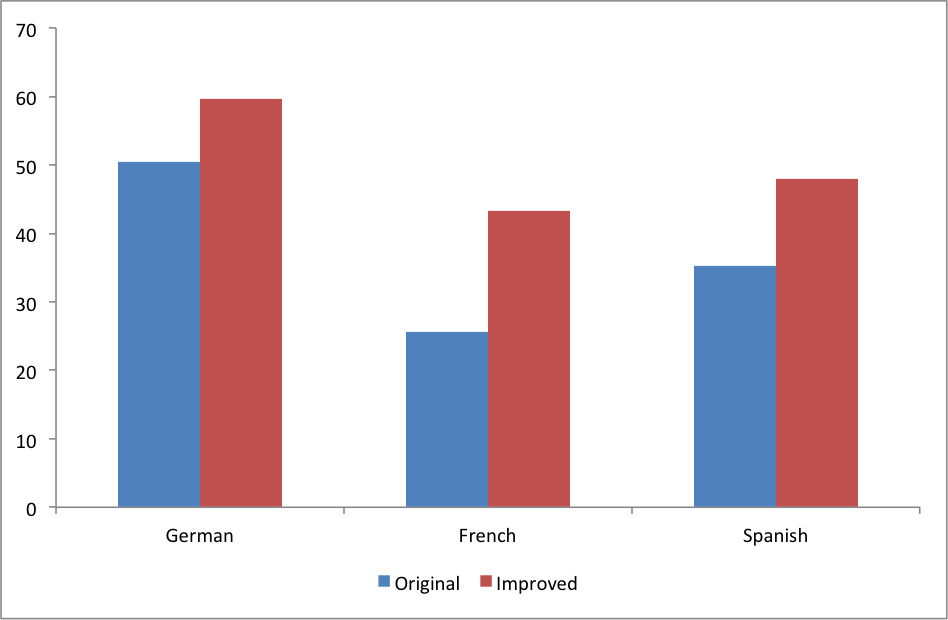
\includegraphics[width=\columnwidth]{multilingual.png}
  \caption{Spearman's correlation for word similarity evaluation on different languages.}
  \label{fig:multi-lang}
\end{figure}

We tested our method on three different languages other than English: German,
French and Spanish. We used the Universal WordNet \cite{deMeloWeikum2009}, which 
is an automatically constructed multilingual lexical knowledge base based on 
WordNet\footnote{\url{http://www.mpi-inf.mpg.de/yago-naga/uwn/}}. 
It contains words connected via different lexical relations to other words both
in and across languages. For a word in a language we only consider links going to
the other words in the same language to construct the word graph.

For German, French and Spanish we were able to retrieve around $87000$, $49000$
and $31000$ words being connected to other words respectively. We used 
RG-65 \cite{Gurevych:2005:USC:2145899.2145986}, WS-353 \cite{Joubarne:2011:CSS:2018192.2018218} 
and MC-30 \cite{Hassan:2009:CSR:1699648.1699665} for German, French and Spanish respectively. 
We trained LSA vectors (\S\ref{sec:lsa}) of length $80$ on WMT-2011 monolingual news corpus for all the 
languages and evaluate word similarity on these tasks before and after enrichment as 
shown in figure~\ref{fig:multi-lang}. The results indicate that our method generalizes across languages.

\section{Qualitative Analysis}

\begin{figure*}[!tb]
  \centering
  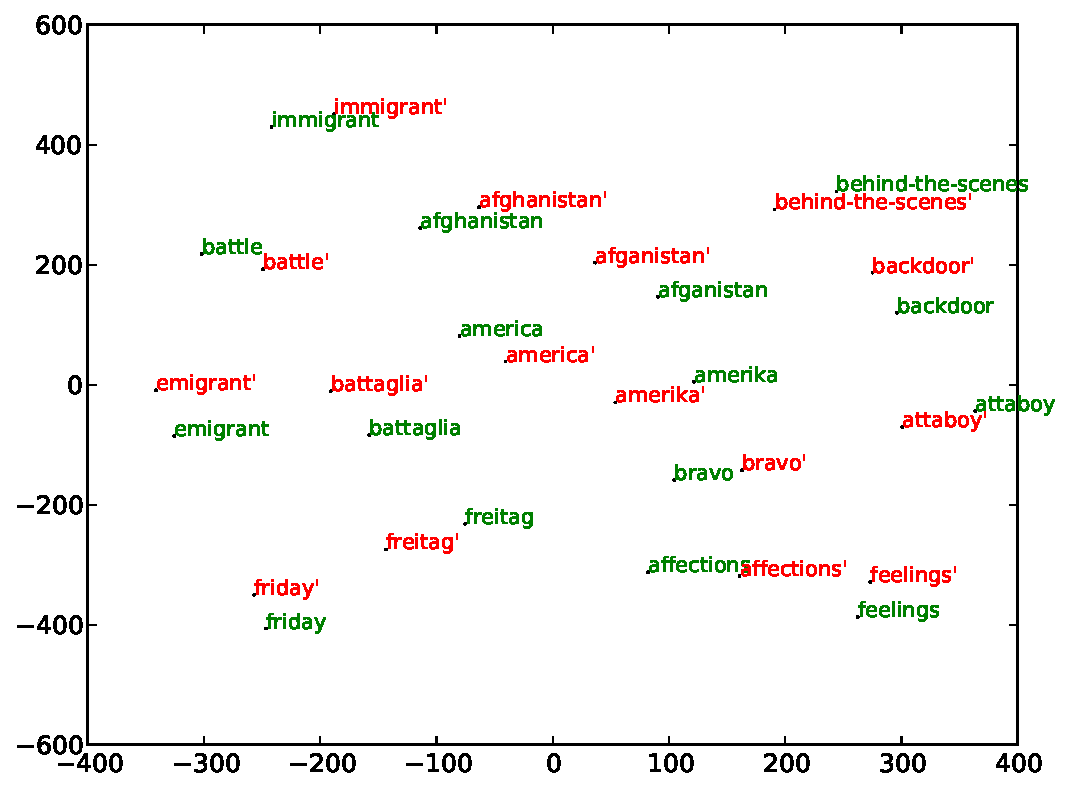
\includegraphics[width=1.75\columnwidth]{img.pdf}
  \caption{Synonymous words or spelling variants of words come closer after enrichment (red) than originally (green).}
  \label{fig:example}
\end{figure*}

To understand how ontological evidence leads to better results in semantic evaluation tasks,
we plot the representations obtained in \S\ref{sec:lsa} both before and after enrichment
of the words that showed significant change in euclidean distance between the two vectors.
We project the vectors onto $\mathbb{R}^2$ using the t-SNE tool~\cite{citeulike:3749741} (cf. figure~\ref{fig:example}). 
Interestingly, most of these words are either minor spelling variations or a rarely used similar
word to one of the frequent words. For example, \textit{amerika} and \textit{afganistan} are 
mis-spelled forms of \textit{america} and \textit{afghanistan} recpectively. Also, 
\textit{behind-the-scenes} and \textit{attaboy} are rare frequency sysnonyms of the words
\textit{backdoor} and \textit{bravo} respectively. We see that these synonyms words are
closer after enrichment (in red) than originally (in green).  


\section{Related Work}

In terms of methodology, the approach we propose is conceptually similar to previous work that leverages graph 
structures to propagate information among semantic concepts~\cite{Zhu:2005:SLG:1104523,10.1109/TPAMI.2007.70765}. Most notably, \newcite{das-smith:2011:ACL-HLT2011} 
construct a factor graph of a semantic lexicon that is used to generalize and apply semantic frames to previously 
unseen types. Graph based belief propagation has also been used to induce POS tags
\cite{Subramanya:2010:EGS:1870658.1870675}.
Our approach is closest to \newcite{das-petrov:2011:ACL-HLT2011} who induce POS tag distribution
for words in a resource poor language through a resource rich language but differs in that we induce
monolingual word vector representations instead of POS tag distributions.

The use of ontological information in training word vectors has been limited. \newcite{alfonseca:2002}, for example, attempt to extend an ontology such as Wordnet with unsupervised and domain-specific information that is yielded by distributional vectors. In contrast, \newcite{gabrilovich:2009} directly construct an ontology of concepts based on the Wikipedia knowledge-graph using a technique called Explicit Semantic Analysis which heavily relies on distributional statistics. \newcite{agirre:2001} enrich the WordNet ontology with topic rather than raw distributional signatures and \newcite{agirre:2013} use the Wordnet graph to perform random-walks that guide a word-sense disambiguation process.
Word vectors have also shown to improve using cross lingual information both during
training \cite{zou-EtAl:2013:EMNLP,hermann2014multilingual} and as a post-processing operation \cite{faruqui-dyer:2014:EACL2014}.  
%and dependency based context \cite{Pado:2007:DCS:1268656.1268658}. 
There have also been disparate attempts at enhancing distributional semantic representations with various sources of non-linguistic information such as images \cite{bruni:2011} and experiential data \cite{andrews:2009}.

Our approach of learning better word vector representations can be seen as an instance of graph based
semi-supervised learning~\cite{Zhu:2005:SLG:1104523,Talukdar:2010:EGS:1858681.1858830} 
where the supervision is derived from the explicit word relations in lexical ontologies. Graph based
learning has also been employed in machine translation \cite{Alexandrescu:2009:GLS:1620754.1620772},
unsupervised semantic role induction \cite{Lang:2011:USR:2145432.2145571}, 
semantic document modeling~\cite{schuhmacher:2014}, 
language generation~\cite{Krahmer:2003:GGR:778822.778825} and
sentiment analysis~\cite{Goldberg:2006:SSA:1654758.1654769}.

\section{Conclusion}

We have proposed a simple and effective method to improve
word vectors (obtained from different models of word representations)
using either automatically or human constructed lexical ontologies
that have explicit information about word relations. We have shown that
ontological information is useful and it can be used both during training
the word vectors or as a post-processing operation. We validated the
applicability of our method across a number of languages and showed that 
performance improvement can be obtained on different types of evaluation tasks.

\bibliography{references}
\bibliographystyle{acl}
\end{document}
